\documentclass[11pt]{article}
\usepackage{enumerate}
\usepackage{fullpage}
\usepackage{fancyhdr}
\usepackage{amsmath, amsfonts, amsthm, amssymb}
\usepackage{graphicx} %for the TM
\setlength{\parindent}{0pt}
\setlength{\parskip}{5pt plus 1pt}
\pagestyle{empty}

\def\indented#1{\list{}{}\item[]}
\let\indented=\endlist

\newcounter{questionCounter}
\newcounter{partCounter}[questionCounter]
\newenvironment{question}[2][\arabic{questionCounter}]{%
    \setcounter{partCounter}{0}%
    \vspace{.25in} \hrule \vspace{0.5em}%
        \noindent{\bf #2}%
    \vspace{0.8em} \hrule \vspace{.10in}%
    \addtocounter{questionCounter}{1}%
}{}
\renewenvironment{part}[1][\alph{partCounter}]{%
    \addtocounter{partCounter}{1}%
    \vspace{.10in}%
    \begin{indented}%
       {\bf (#1)} %
}{\end{indented}}

%%%%%%%%%%%%%%%%% Identifying Information %%%%%%%%%%%%%%%%%
%% This is here, so that you can make your homework look %%
%% pretty when you compile it.                           %%
%%     DO NOT PUT YOUR NAME ANYWHERE ELSE!!!!            %%
%%%%%%%%%%%%%%%%%%%%%%%%%%%%%%%%%%%%%%%%%%%%%%%%%%%%%%%%%%%
\newcommand{\myname}{Karan Sikka}
\newcommand{\myandrew}{ksikka@andrew.cmu.edu}
\newcommand{\myhwname}{Assignment 10}
\newcommand{\myrecitation}{E}
%%%%%%%%%%%%%%%%%%%%%%%%%%%%%%%%%%%%%%%%%%%%%%%%%%%%%%%%%%%

\begin{document}
\thispagestyle{plain}

\begin{center}
{\Large \myhwname} \\
\myname \\
\myandrew \\
\myrecitation \\
\today
\end{center}
\begin{question}{I Wish I Could Use The Church-Turing Thesis}
First, I give a high level description of the turing machine.
Second, I go more in detail about it's functionality.
Third, I give a full formal definition and diagram of the Turing Machine $M$.

\textbf{High Level Detail}
\begin{enumerate}
\item If the tape is empty, we will read a \textvisiblespace. In this case, we 
should move to the reject state and halt immediately.

Else, we have a valid input, because it will start with either 0 or 1.
The result of adding 1 to a number in binary may have at most 1 more bit than
it originally had, so we shift all bits one space to the right on the tape to 
make room for that bit. We fill the leftmost cell with $\#$. 

\item The process of shifting all bits over one will put the head at the least 
significant bit of the binary string. Starting from the least significant bit 
and moving left, the algorithm 
to add one to a binary number is as follows.

Adding one requires flipping the rightmost bit.

If you're flipping a 0 to a 1, you can stop. Addition is done.
If you're flipping a 1 to a 0, you need to flip the bit to the left of this 
bit.
Then, recursively, you need to continue flipping leftwards until you flip a 0.

If the leftmost bit is 0, you make it a 1 and change the $\#$ to the left of it a 0.
If the leftmost bit is 1, you make it a 0 and change the $\#$ to the left of it a 1.

\item  Move all the way left to the $\#$ and change it to a 0. 
Transition to our accept state and halt.
\end{enumerate}

\textbf{Medium Level Detail}\\
The string goes in the TM with the head on the leftmost bit. It then goes into
a set of states which will write $\#$ and willshift all bits over to the right one state.
On the last shift, it moves right, and then left to bring the head on the rightmost bit.

It then goes left into the addition/bitflip mechanism. It implements the bit flipping
described in step 2 above. Eventually the head will reach the leftmost bit, and it moves
right because it is unknown what is to the left of the left most bit. Then the head
moves left to be on the leftmost bit, to satisfy the problem statement.

\textbf{Formal TM}\\
$Q = \{q_{start}, q_{accept}, q_{reject}, q_{copy0}, q_{copy1}, q_{bound}, q_{add}, q_{shift}, q_{end} \}$\\
$q_{start}$ is the start state.\\
$q_{reject}$ is the reject state.\\
$\Sigma = \{0, 1\}$.\\
$\Gamma = \{0, 1, \#, \sqcup \}$.\\

$M = (Q, \Sigma, \Gamma, \delta, q_{start}, q_{accept}, q_{reject})$.
The $\delta$ transitions are shown explicitly with a finite state control 
below. 
Each transition/arrow is represented as a 3-tuple containing character 
read, character wrote, and direction. 

\scalebox{0.17}{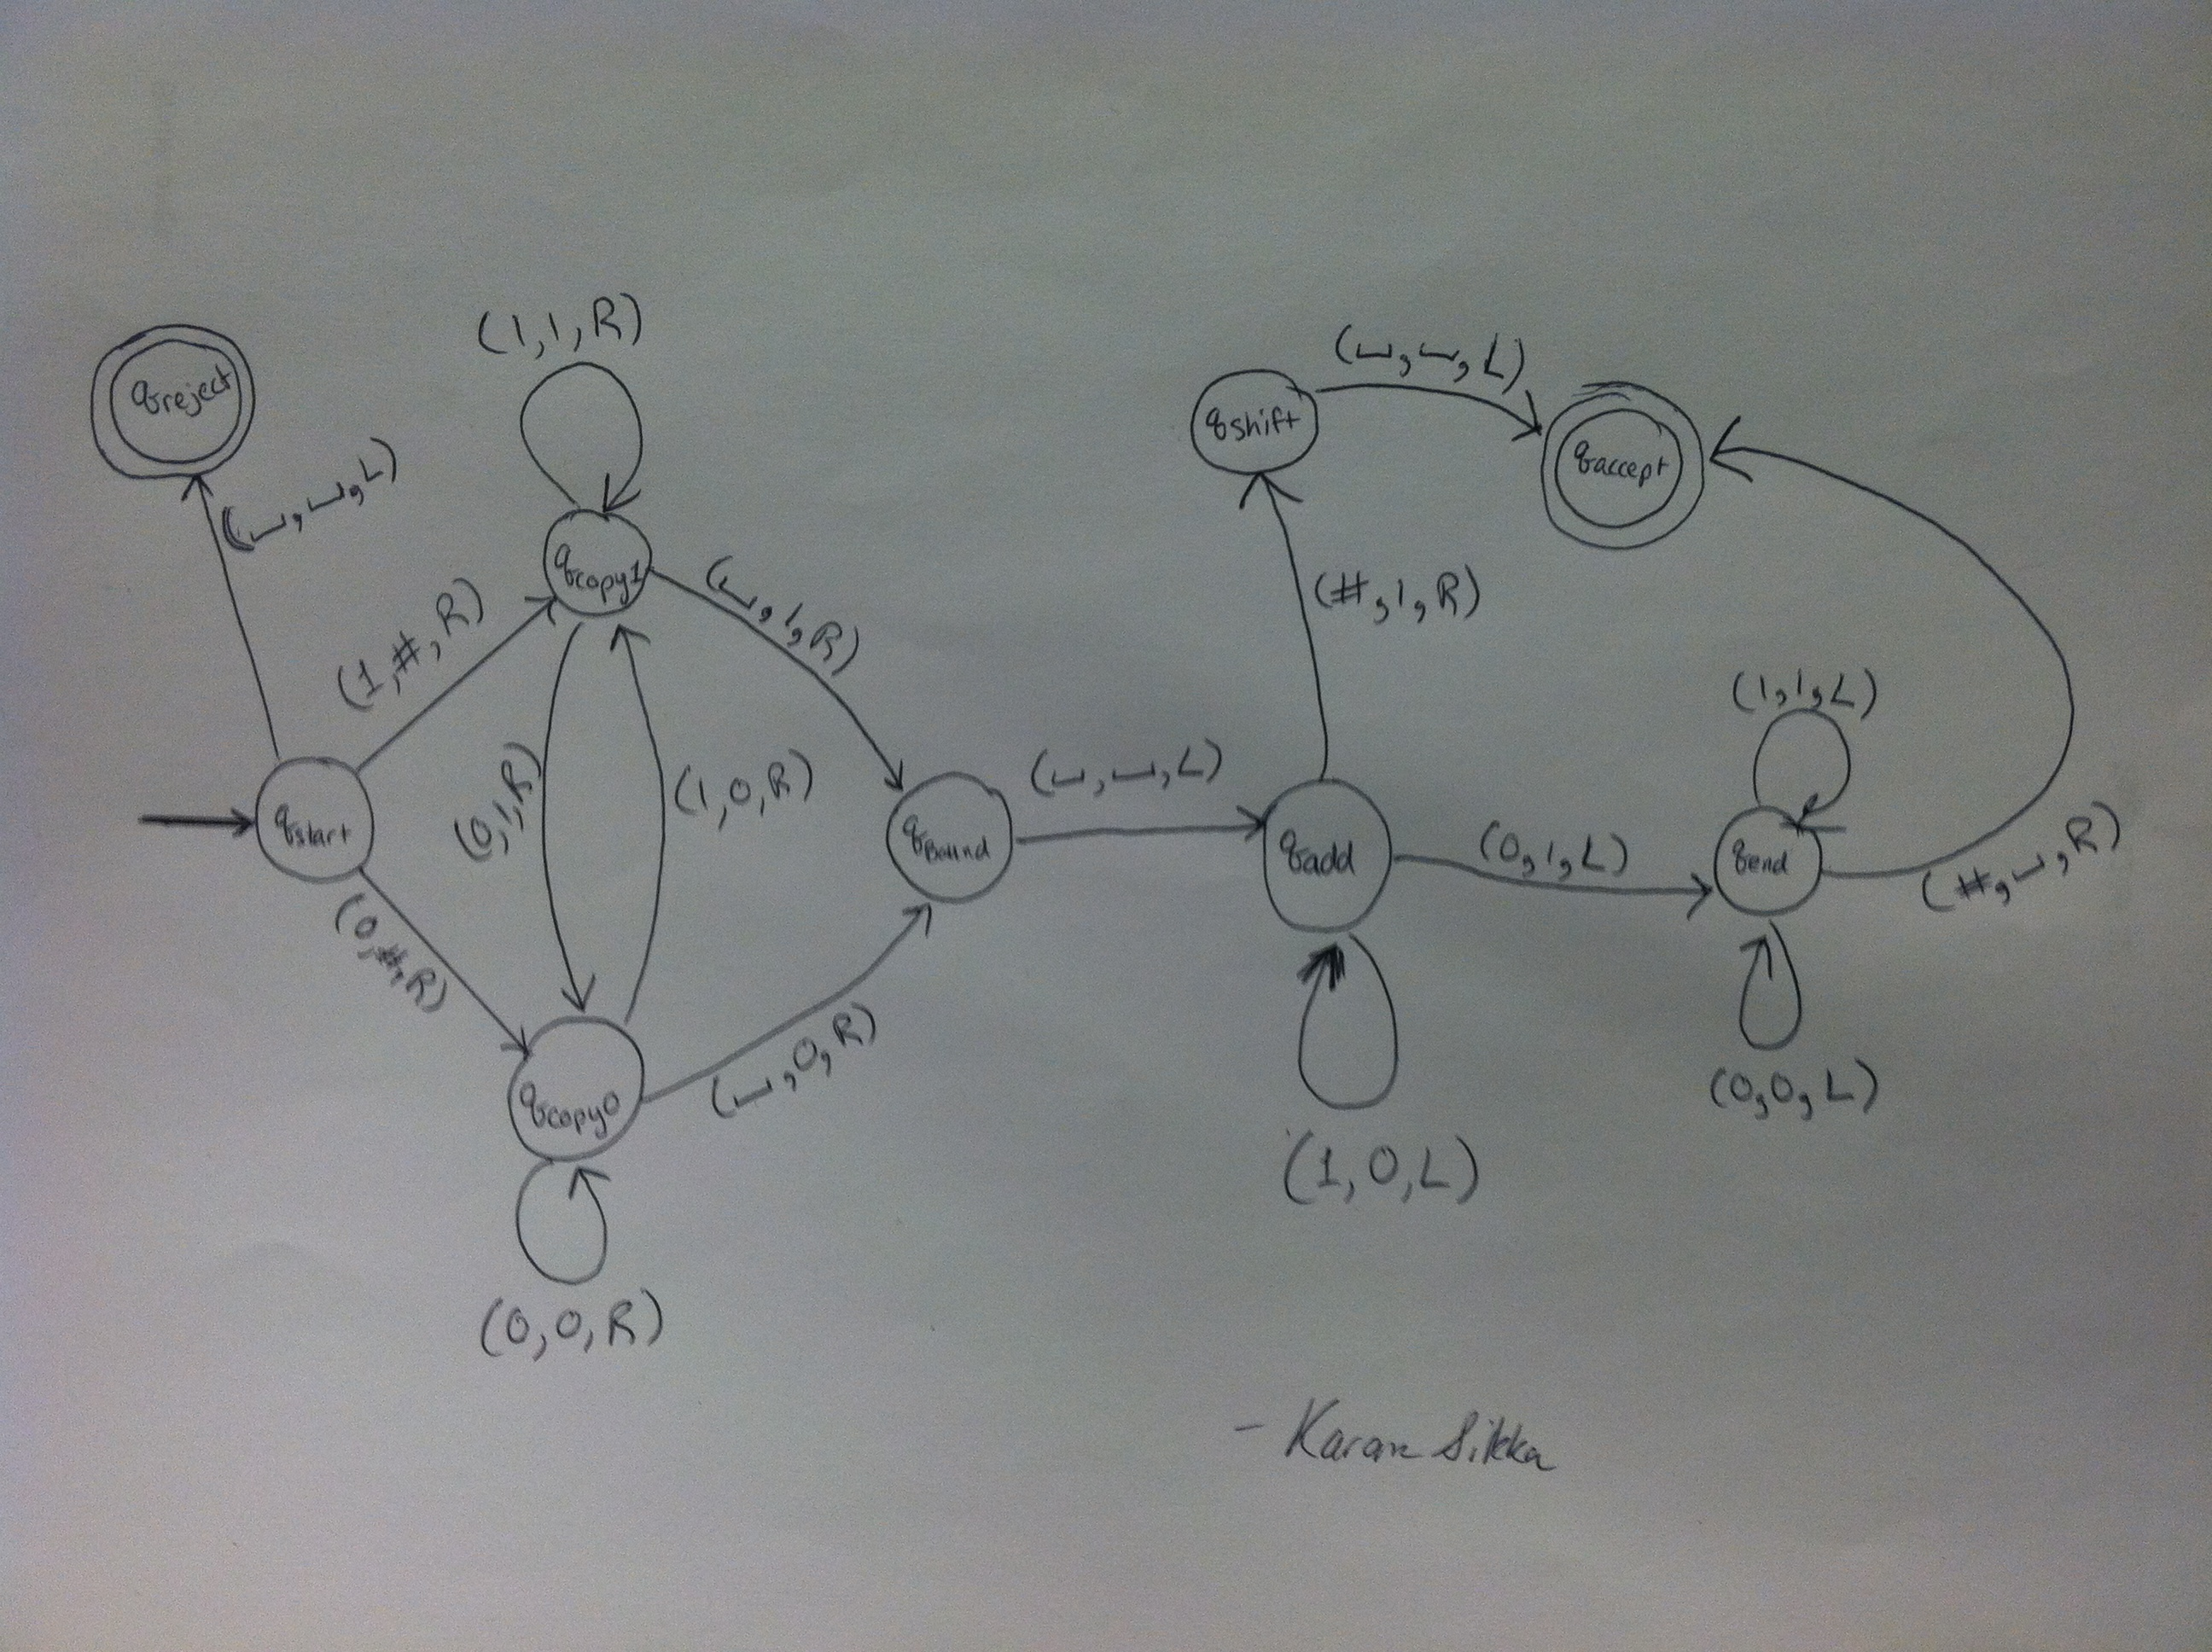
\includegraphics{tm.jpg}}
\end{question}
\begin{question}{Computers Have Printers!}
\begin{enumerate}
\item \textbf{WTS} a language $L$ is printable iff it's acceptable: $L$ printable $\iff L$ acceptable.

\textbf{Proof} for forwards implication\\
If $L$ is printable, then there a TM $M$ which prints $L$. AFSOC that $L$ is not acceptable. 
Therefore there is a string in $L$ such that $M$ rejects $s$, so $s$
isn't completely printed since $M$ halts before fully processing it.
This is a contradiction, because $L$ is printable means that for all $s$  in $L$, 
$M$ is able to transition through \emph{all} its states and thus can print all strings in $L$ completely. \qed

\textbf{Proof} for reverse implication\\ 
If $L$ is acceptable then there exists a TM $M$ such that it halts on all inputs in $L$.
Therefore there exists a transition $\delta$ which processes all strings in $L$ through $M$ and reaches an accept state.
Therefore, all strings in the language can be processed and printed completely by $M$, so $L$ is printable. \qed

\item \textbf{WTS} $L$ is not acceptable where $L = \{\langle M, x\rangle | M(x)$ does not accept$\}$.\\
\textbf{Proof} AFSOC $L$ is acceptable, which means that there exists a TM $M$ which accepts strings
in $L$. Therefore $M(s)$ accepts for $s \in L$. 
Now, we construct $L$ for $M\langle M, x\rangle$ such that $M(x)$ does not accept. However, this 
is clearly a contradiction if $L$ is acceptable because then $M$ must accept inputs $\langle M, x\rangle$.

\item \textbf{WTS} $L = \{ \langle M \rangle \mid M \textbf{ has a pointless state } \}$ is undecideable.
\textbf{Proof} AFSOC $L$ is decidable. Then there exists a TM $U$ that decides $L$.

Construct a TM $M'$ which takes $\langle M, x\rangle$ as input such that
\begin{enumerate}
\item visits all states in $M'$ except state $q_{k}$
\item simulates $M(x)$ 
\item transitions to state $q_{k}$ 
\item terminates
\end{enumerate}
Recall that by our assumption we have a machine $U$ which can decide whether 
$M'$ has a pointless state or not. Hence there are two cases: $U$ accepts or 
rejects $\langle M' \rangle$. In the case that $U(\langle M' \rangle)$ accepts, 
$M(x)$ terminated. In the case $U(\langle M' \rangle)$ rejects, 
we know that $q_{k}$ is a pointless state. Note that we are supposed to visit $q_{k}$ when $M(x)$ terminates.
Since we never visit it, $U(\langle M' \rangle)$ rejecting implies that $M(x)$ loops.
Hence, we see that $U$ is essentially a halting oracle, which can't possibly exist, and we have
reached a contradiction.
\end{enumerate}
\end{question}
\begin{question}{LambdaLaTeX}
\end{question}
\end{document}
